\documentclass[11pt]{article}

\usepackage{fancyhdr}
\usepackage{extramarks}
\usepackage{amsmath}
\usepackage{amsthm}
\usepackage{amsfonts}
\usepackage{tikz}
\usepackage{graphicx}
\usepackage{enumitem}
\usepackage[plain]{algorithm}
\usepackage{algpseudocode}
\usepackage[normalem]{ulem}
\usepackage{hyperref}
\usepackage{xcolor}
\usepackage{caption}
\usepackage{subcaption}
\usepackage{listings}% http://ctan.org/pkg/listings
\usepackage{array}
\newcolumntype{L}[1]{>{\raggedright\let\newline\\\arraybackslash\hspace{0pt}}m{#1}}
\lstset{
  basicstyle=\ttfamily,
  mathescape
}

\hypersetup{
    colorlinks=true,
    linkcolor=blue,
    filecolor=magenta,
    urlcolor=blue,
}

\usetikzlibrary{automata,positioning}

\topmargin=-0.45in
\evensidemargin=0in
\oddsidemargin=0in
\textwidth=6.5in
\textheight=9.0in
\headsep=0.25in

\linespread{1.1}

\pagestyle{fancy}
\lhead{
\includegraphics[width = 17pt]{logo.jpg} \hmwkAuthorName\: (\hmwkAuthorEmail)}
\rhead{\hmwkTitle}
% \rhead{\firstxmark}
\lfoot{\lastxmark}
\cfoot{\thepage}

\renewcommand\headrulewidth{0.4pt}
\renewcommand\footrulewidth{0.4pt}

\setlength\parindent{0pt}

\setcounter{secnumdepth}{0}
\newenvironment{homeworkProblem}[1][-1]{
    \ifnum#1>0
        \setcounter{homeworkProblemCounter}{#1}
    \fi
    \section{Problem \arabic{homeworkProblemCounter}}
    \setcounter{partCounter}{1}
    \enterProblemHeader{homeworkProblemCounter}
}{
    \exitProblemHeader{homeworkProblemCounter}
}

\newcommand{\hmwkTitle}{Software Design Specification}
\newcommand{\hmwkClass}{CSE 403 (Wi16)}
\newcommand{\hmwkAuthorName}{Check Your Bias}
\newcommand{\hmwkAuthorEmail}{checkyourbias@u.washington.edu}

\title{
    \vspace{2in}
    \textmd{\textbf{\hmwkClass:\ \hmwkTitle}}\\
    \vspace{0.1in}\large{\textit{\hmwkClassInstructor\ \hmwkClassTime}}\\
    \author{\textbf{\hmwkAuthorName\ $\vert$ \hmwkAuthorCSE\ $\vert$ \hmwkAuthorId}}
}

\date{}

\renewcommand{\part}[1]{\textbf{\large Part \Alph{partCounter}}\stepcounter{partCounter}\\}

\DeclareMathOperator*{\argmin}{arg\,min}

\DeclareMathOperator*{\argmax}{arg\,max}

\begin{document}

\section*{System Architecture}

The Check Your Bias (CYB) system architecture is split into four major modules at a high level, the modules are:

\begin{enumerate}[nolistsep]
    \item Firebase
    \begin{enumerate}
        \item Responsible for storing the actual data.
    \end{enumerate}
    \item Data Model
    \begin{enumerate}
        \item Responsible for providing an interface between the Firebase database it’s client applications in the form of concrete data models.
    \end{enumerate}
    \item Mobile Client
    \begin{enumerate}
        \item Responsible for providing a user interface for users to interact with the system. Implemented with React components.
    \end{enumerate}
    \item Crowd Source Approval Utility
    \begin{enumerate}
        \item Responsible for approving or denying crowd sourced content uploaded to the system through the Mobile Client
    \end{enumerate}
\end{enumerate}

We will now describe each module in detail.

\subsection*{Firebase}

Firebase provides one key features we will use for CYB: data storage. We will use the data storage feature to store all the CYB data in relational form according to the UML diagram provided in this document. In place of a full server, we will utilize Firebase to fetch data via our Data Model module. We can then implement functionality to pre-process our data before returning it to the client application.\\

From a user's perspective, this module is hidden other than the views we provide to the data.

\subsection*{Data Model}

The data models are responsible for abstracting access to the Firebase database in a unit-testable way. They are a direct reflection of the data UML diagrams provided in this document. The data models are then used by the Mobile Client and Crowd Source Approval Utility to access and write to the Firebase database. From a technical perspective, this module will consist of a group of TypeScript classes which encapsulate the raw data provided by fetching the appropriate data from the Firebase database. The data model also will handle any preprocessing of the data into more application friendly forms. For example, the data model can produce a ranking list of candidates from processing the raw Firebase data.\\

Again, from a user's this part of the system is hidden. The Mobile Client will interact with this module directly to produce the views the user will experience.

\subsection*{Mobile Client}

The mobile client is a user centric module. The mobile client, written in web technologies, will provide a view to the user to interact with our system. From a technical perspective, this module will be implemented as a collection of React components which are fed data through the Data Model module by utilizes the various TypeScript classes provided by it.\\

From a users perspective, the mobile client will reside as a native phone application on iOS and Android. The native application, generated by Phonegap, will consist of a webview that displays the application generated by the composition of React components. The user will be able to contribute crowd data, and participate in the CYB system via this module.

\subsection*{Crowdsource Approval Utility}

The Crowd Source Approval Utility (CSAU) will provide administrative access to the Firebase database to approve or deny submissions to the crowd source data set. From a technical perspective the CSAU will be a NodeJS command-line utility which will interact, via the Data Model module, with the Firebase database. From a user’s perspective (the user in this case is an administrator), the command-line utility will allow listing pending-approval submissions and approved submissions. It will also allow administrators to deny and approve submissions.

\section{Interfaces Between Modules}

The major interfaces of CYB generally exist with respect to accessing data. The interfaces are as follows:

\subsection*{Mobile Client \& Data Model}

The Mobile Client module will interact with the Data Model module to obtain data to display to the user. It will also interact with the Data Model to store user preferences, political profile additions, and crowd sourced data. This interaction from a technical perspective will involve constructing TypeScript classes exposed by the Data Model module. These classes can be constructed by JSON object, or by a simple constructor. Once constructed, the mobile client can use the model to fetch or store data. The Data Model will then take these actions and interact with the Firebase database.

\subsection*{Crowdsource Approval Utility \& Data Model}

Similar to how the Mobile Client functions, the Crowd Source Approval Utility will interact with the Data Model module to obtain and change approval queues in the Firebase database. Since the Crowd Source Approval Utility is also written in JavaScript (similar to the Mobile Client), the interface will similarly consist of constructing TypeScript classes, and invoking interfaces to fetch and save data.

\subsection*{Firebase \& Data Model}

Finally, there will be an interface between the Data Model and the Firebase database. The interface will execute with HTTP REST requests which will fully specify the interactions between the models and the database. For example, if storing a new user object, the Data Model module will use the information specified by the clients of the Data Model (such as username), to generate and execute a request to the Firebasee database for storage.

\section*{Alternative Designs}

\subsection{Facebook Login}

Instead of using Facebook authentication in order to log in to CYB, we also considered building out our own authentication system or using multiple systems such as Google+ alongside Facebook. While using Facebook authentication makes building on the developer’s side significantly easier, it also ensures security. It trades off ease of access to existing Facebook users for the pain of signing up for Facebook and the loss of a potential user who is vehemently against Facebook. We chose to use Facebook over a multi-system login step because it opens up possibilities for the future in case we want to further personalize CYB with some of Facebook’s social functionalities.

\subsection{Firebase Vs. Parse}

We strongly considered using Parse over Firebase. While they offer similar features, Parse allows for everything we need but is also backed by Facebook which we chose as our login feature so the integration is likely better. Firebase offers real time data as its main benefit over Parse but this is a feature that is most likely unimportant for the purposes of CYB. However, it was recently announced that Parse would be discontinued at the beginning of next year. We chose to use Firebase because it offers similar features to Parse but the skills and knowledge we would develop while using it would persist and so we would not have to migrate platforms if the project continued further.

\section{Data Storage}

\begin{itemize}[nolistsep]
    \item[] For each \textbf{user}:
    \begin{itemize}[nolistsep]
        \item Facebook Id
        \item Issues they have submitted
        \item Issues they have responded to
    \end{itemize}

    \item[] For each \textbf{candidate}:
    \begin{itemize}[nolistsep]
        \item A unique Id
        \item Their name
        \item A source for users to get more information about this candidate
    \end{itemize}

    \item[] For each \textbf{issue}:
    \begin{itemize}[nolistsep]
        \item A unique Id
        \item The issue content, i.e. a quote from a candidate
        \item A source
        \item Candidate opinions where applicable
    \end{itemize}
\end{itemize}

\vspace{10pt}

The schemas of the objects we will be using (represented in Orderly format), which reflect how our objects will be stored, are as follows:\\

\begin{centering}
\begin{tabular}[t]{l|l}
    \begin{minipage}[t]{3.75in}
        \begin{verbatim}
User {
    integer userId;
    string email;
    string firstName;
    string lastName;
    integer age;
    integer gender;
    boolean admin;
    boolean hasSeenHelpText;
    array {
        integer;
    } submittedIssueIds;
    map { integer => integer } ratedIssues;
    map { integer => integer } categoryWeights;
}
        \end{verbatim}
    \end{minipage}
    &
    \begin{minipage}[t]{2.85in}
        \begin{verbatim}
Category {
    integer categoryId;
    string categoryName;
    string description;
    array {
        integer;
    } issues;
}
        \end{verbatim}
    \end{minipage}\\[10pt]
    \hline
    \begin{minipage}[t]{3.3in}
        \begin{verbatim}
Issue {
    integer issueId;
    string mainText;
    array {
        string;
    } sources;
    map { integer => integer } candidates;
    array {
        integer;
    } category;
    array {
        integer;
    } submitters;

    integer seenByCount;
    integer skipCount;
    map { integer => integer } ratings;
    integer flagCount;

    boolean approved;
}
        \end{verbatim}
    \end{minipage}
    &
    \begin{minipage}[t]{2.85in}
        \begin{verbatim}
Candidate {
    integer candidateId;
    string name;
    string affiliatedParty;
    map { integer => integer } issues;
    string website;
}
        \end{verbatim}
    \end{minipage}
\end{tabular}

\end{centering}

\section{Design Assumptions}
\vspace{-10pt}
We were very careful in our system architecture design to limit places where we are making general assumptions or constricting opportunities for the system to adjust and react to new factors. For example, we carefully designed the system such that it is not dependent on the setting for elections presented in the application. While we mainly had presidential elections in mind when thinking about the design, we left it flexible enough to support other election cycles in the federal level, as well as the state, county, city, and local jurisdictions. In fact, our system is not even reliant on the elections taking place in the United States, or on elections being political at all. In fact, the same exact system architecture design will serve us well when comparing candidates for a 5th grade hallway monitor in Finland! We did however, make a few small assumptions in other areas. One of those concerns the behavior of our users. We are assuming that every user of the platform will behave in a similar fashion by voting on their opinion on issues to some extent. If users chose not to vote at all, then our platform will not adjust well and not have enough data available to provide the user with new information or an informed decision on their possible political affiliations. Secondly, we are assuming that users have informed opinions and preexisting knowledge about issues that may come up in the election discussion. We currently do not have any plans to implement features that will help explain the significance or meaning of the issues presented to the users.

\vspace{-16pt}

\section{Diagrams}

\begin{centering}
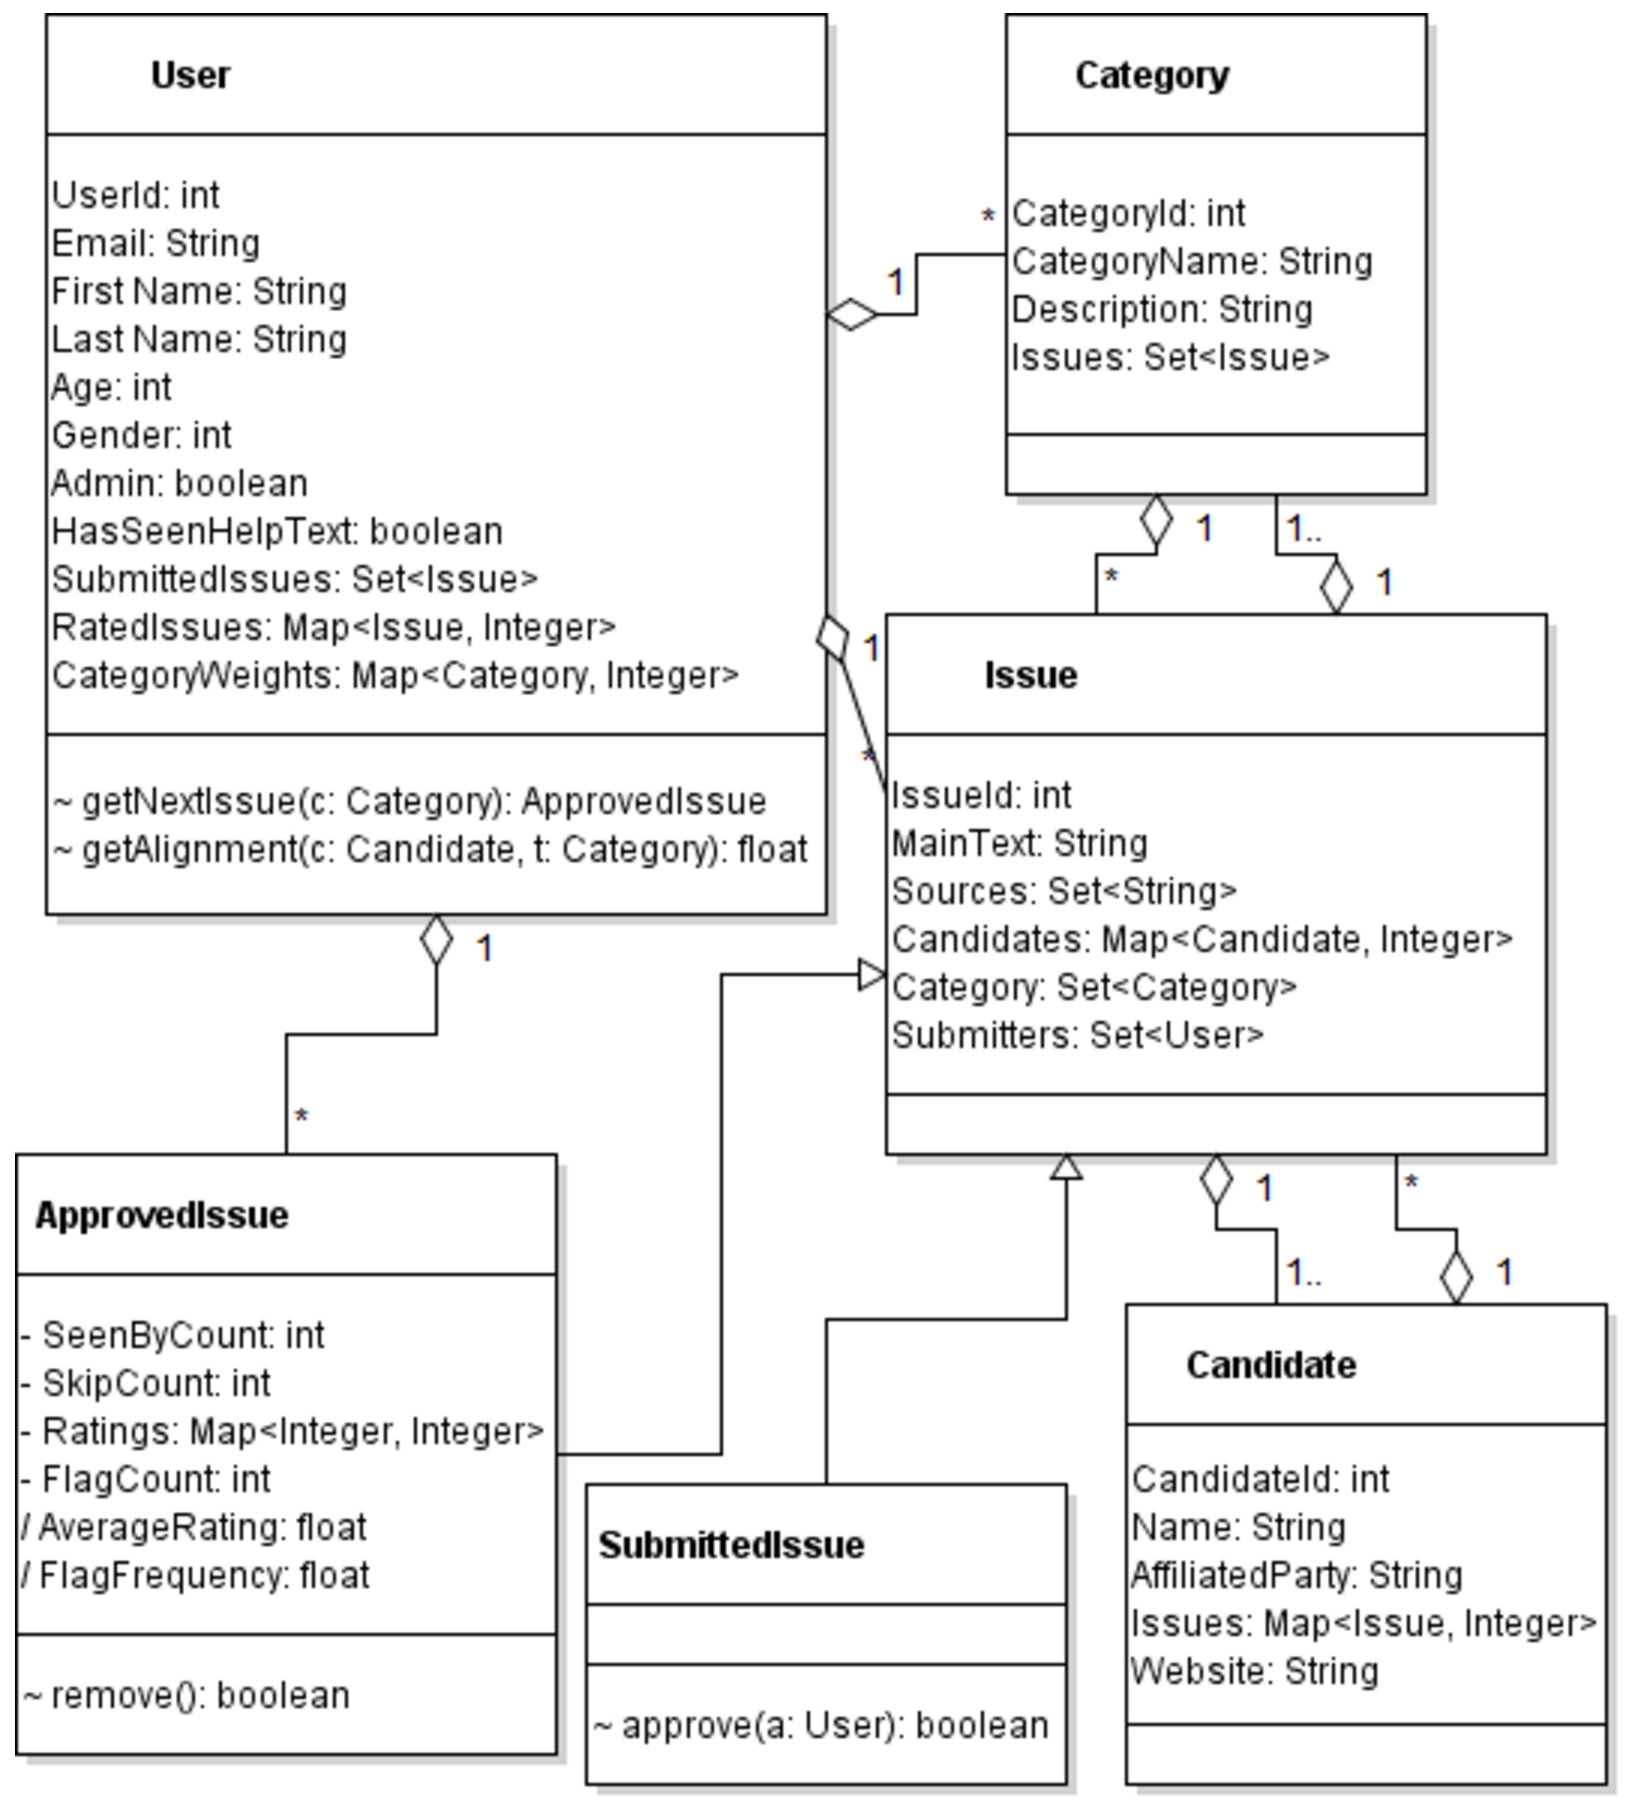
\includegraphics[width = 0.70\textwidth]{uml_diagram.png}

\end{centering}

\begin{centering}
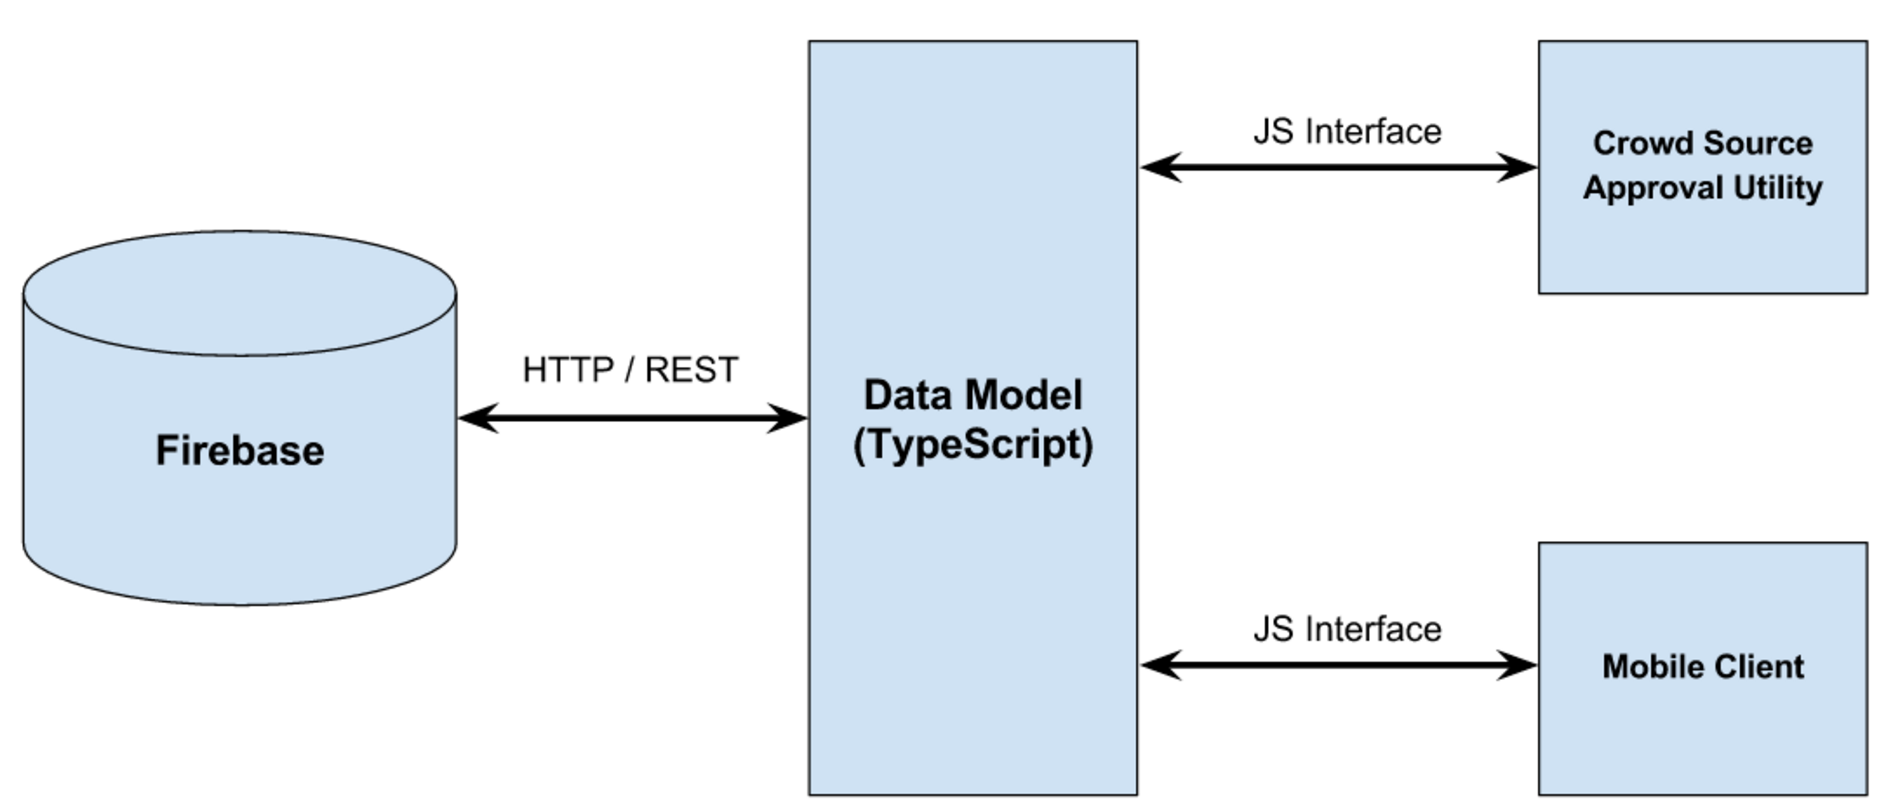
\includegraphics[width = \textwidth]{backend_model.png}

\end{centering}

\newpage

\section{Sequence Diagrams}

\subsection{User Voting}

\begin{centering}
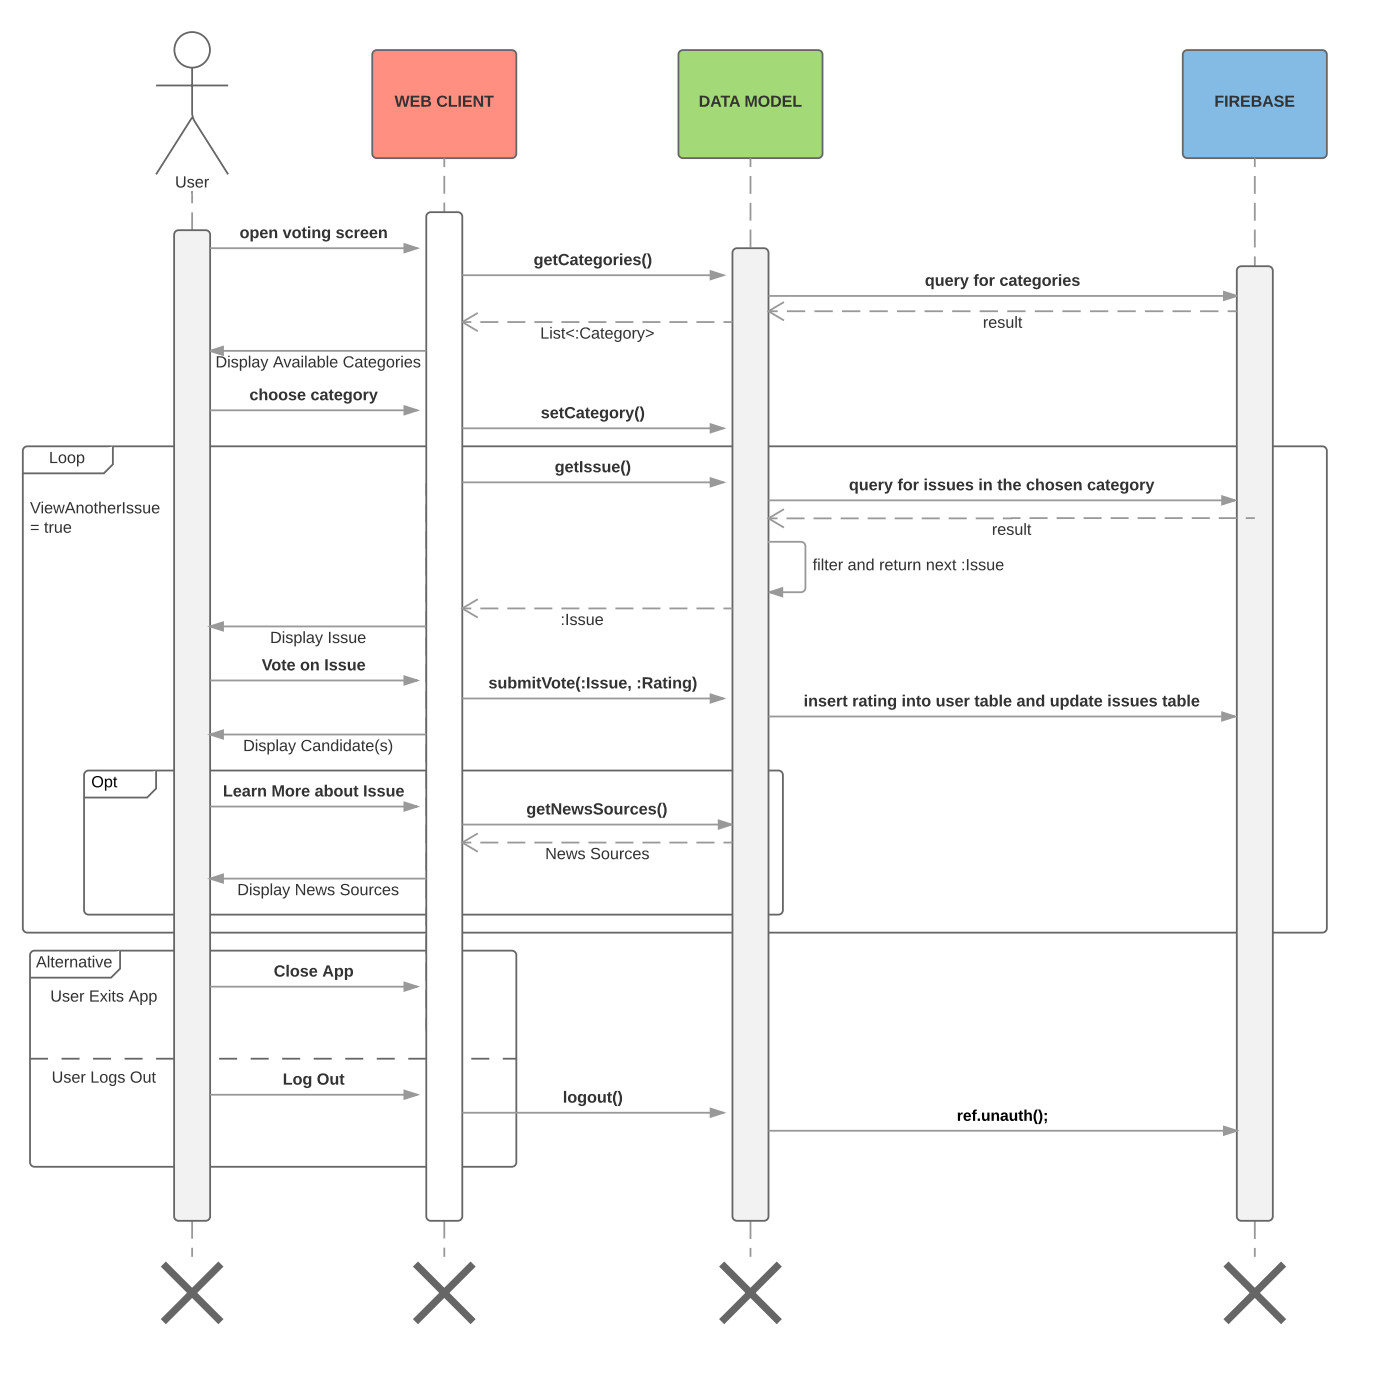
\includegraphics[width = 0.7\textheight]{sonja.png}

\end{centering}

\newpage

\subsection{Crowdsourcing}

\begin{centering}
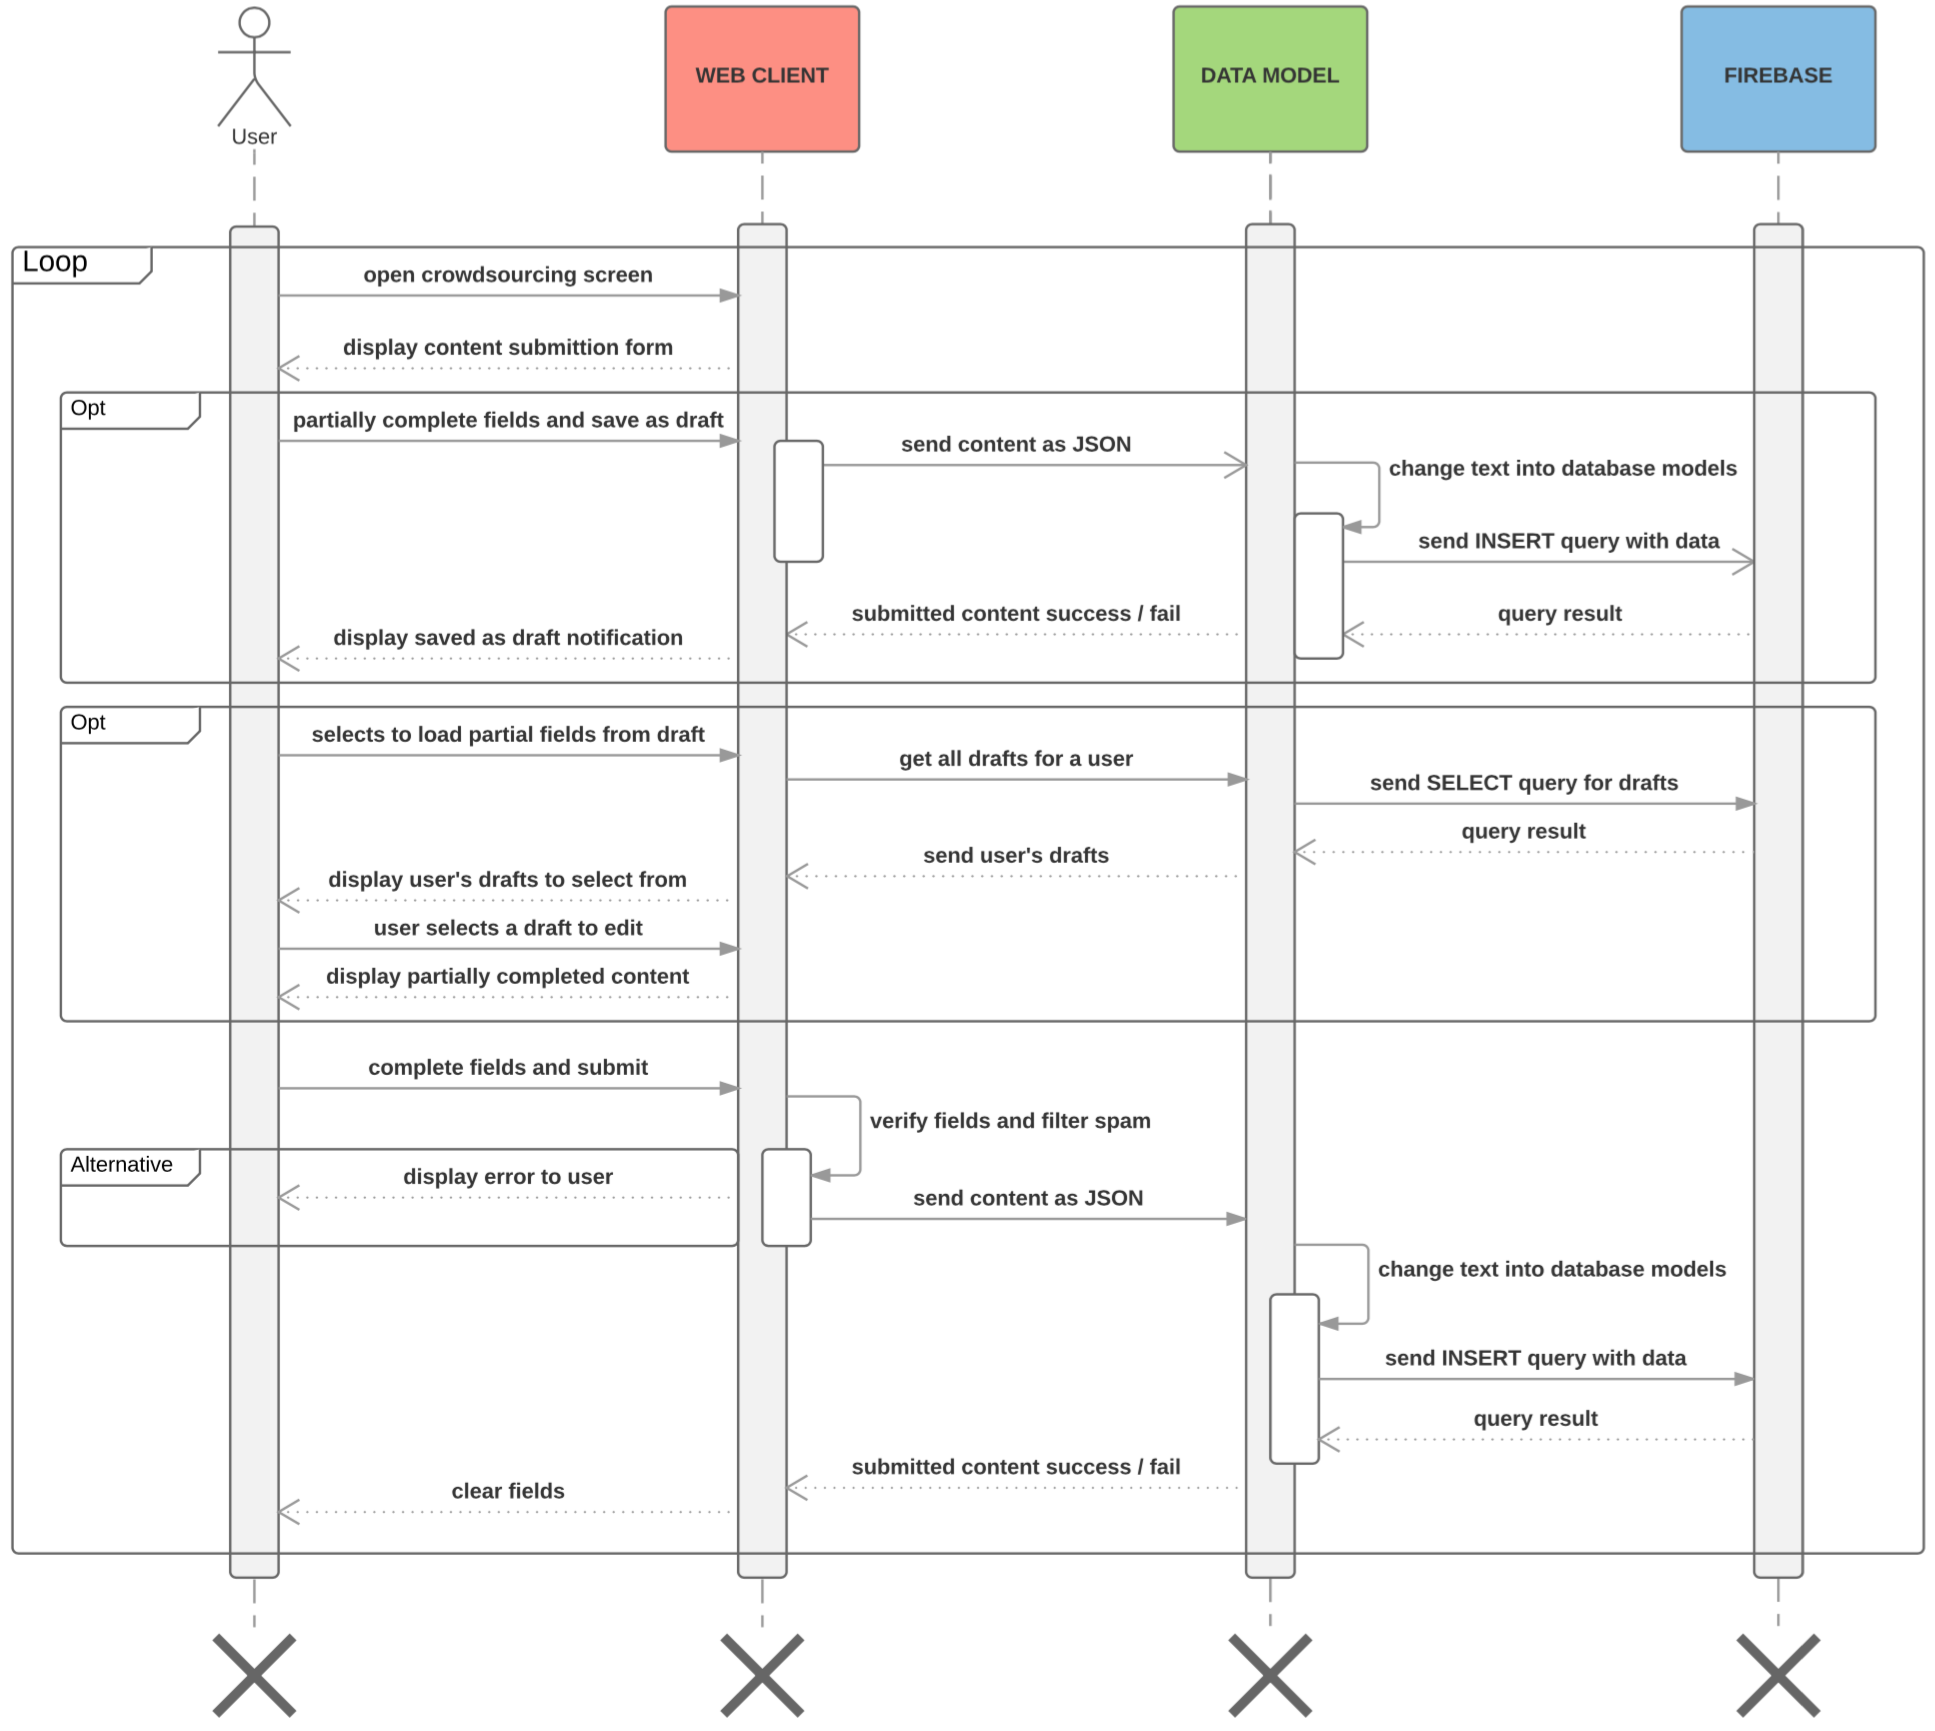
\includegraphics[width = 0.7\textheight]{ryan.png}

\end{centering}
\newpage
\section{Process}

\subsection{Risk Assessment}

\begin{enumerate}[nolistsep]
    \item \textbf{Content}\\
        \textbf{Likelihood}: Medium\\
        \textbf{Impact}: High\\
        \textbf{Summary / Evidence}: Content is a major component of Check Your Bias and it is incredibly important that this information be both accurate and complete. The content will be directly related to the overall quality of our application.\\
        \textbf{Overall Plan}: We plan to review all content that is put into our app as a team in the beginning. That means that before content can show up in the feed for users, it has to be approved by admins who will check the accuracy and completeness.\\
        \textbf{Detection}: This was discussed about, but all content will be moderated before it can show up in a user's feed.\\
        \textbf{Mitigation Plan}: Should this occur, users can report something as incorrect with a few simple taps when voting on a topic or issue.\\[-10pt]

    \item \textbf{Crowdsourcing}\\
        \textbf{Likelihood}: Medium\\
        \textbf{Impact}: Medium\\
        \textbf{Summary / Evidence}: Crowdsourcing will allow the product to grow significantly and provide a platform for many people to share their knowledge and expertise in the topic, but it also produces significant challenges. Content that users supply to the app must be vetted and screened thoroughly and pass quality guidelines. It will be difficult balancing the effort and efficiency of undergoing this screening process.\\
        \textbf{Overall Plan}: All content must be initially reviewed by moderators, but in order for this to scale there must exist a limit to how much one can spend on a single topic before making a decision. \\
        \textbf{Detection}: Moderators will need to be careful that the time spent approving or disapproving content is of high quality so that a short amount of time can be spent on each submission while also insuring that only high quality content is approved.\\
        \textbf{Mitigation Plan}: Should this fail to happen, then users will be able to flag content for review (as discussed in the previous risk).\\[-10pt]

    \item \textbf{Content Creation}\\
        \textbf{Likelihood}: Medium\\
        \textbf{Impact}: Medium\\
        \textbf{Summary / Evidence}: A major feature of our end product is providing users the option to answer a set of questions that will help the product guide them towards a candidate whose opinions match their own. Since this process and criteria will at first be created manually by us, the creators of the products, there is a risk that our bias or incomplete understanding of the political situation will impact the quality of this initial survey and will thus degrade the overall quality of the product.\\
        \textbf{Overall Plan}: In addition to all content being approved by a set of moderators, each moderator should carefully consider whether the submission is inherently bias towards a particular candidate or viewpoint. \\
        \textbf{Detection}: Detection can happen in 2 places: another moderator will catch it before it is approved or a user will flag the content.\\
        \textbf{Mitigation Plan:} If a moderator finds content to be inherently biased, then they may edit the content to be better suited for the content feed.\\[-10pt]

    \item \textbf{Lack of Engagement}\\
        \textbf{Likelihood}: Low\\
        \textbf{Impact}: High\\
        \textbf{Summary / Evidence}: A user may come into our app and only answer a few questions and then stopping. This does not give us enough evidence to make any conclusions about who the user most closely relates to in terms of the candidates. \\
        \textbf{Overall Plan}: We will display a message saying that there is not enough information yet to make any conclusions about the user's political views if the user tries to access the analysis page. \\
        \textbf{Detection}: This can be detected if the user tries to access his or her political profile page before they have ranked enough topics or issues.\\
        \textbf{Mitigation Plan}: The main way of mitigating this risk is to tell the user they must answer X questions or topics before we have enough information to make a conclusion about their political profile. If a user has already taken the time and effort to download our application, then it is likely that asking them to spend a few more minutes rating topics will not deter them away from CYB. Unfortunately, it would be incredibly difficult to make any conclusions based on such little data.\\[-10pt]

    \item \textbf{Rated Content}\\
        \textbf{Likelihood}: Medium\\
        \textbf{Impact}: Medium\\
        \textbf{Summary / Evidence}: As a user rates content in his or her feed, it is likely that they will encounter a category that is of not much importance to them. For example, if I have an extreme bias against Trump and disagree on every single one of his viewpoints -- then it is highly unlikely for me to have my views changed (the main idea of CYB is to help educate voters about their views and how they relate to the candidates' views). If I rate a quote of Trump's that happens to be one of his main campaign points as ``Highly Disagree'', then I probably won't agree with many of his other points.\\
        \textbf{Overall Plan}: This can be mitigated by using a user's vote on a topic as an indicator whether he or she agrees with a candidate before the user's political profile is made. The server can then send topics to the user that help complete the profile rather than sending more topics on someone or something that they do not care for.\\
        \textbf{Detection}: Detection of this risk is a difficult task. We can look at the likelihood of a user voting ``Highly Disagree'' on a topic given that they also voted ``Highly Disagree'' on this other topic and use this as a metric in determining whether or not to show them.\\
        \textbf{Mitigation Plan}: Largely discussed above, we want to show users topics that help complete our political profile of them. This means that we should have a diverse set of content that can be utilized to help find the right topics to present to the user.
\end{enumerate}

\subsection{Project Schedule}
\newcommand{\tabitem}{~~\llap{\textbullet}~~}
\begin{tabular}[t]{|L{1.45in}|L{1.45in}|L{1.45in}|L{1.45in}|}
    \hline
    \textbf{Team Goals for} & \textbf{Front End Team} & \textbf{Back End Team} & \textbf{Full Stack Team}\\
    \hline
    \textbf{January 26th} & Learn React & Learn Firebase & Crowdsource Design\\
    \tabitem Submit Software Design Specification & \textbf{Aaron} - Modules and Interfaces, UML & \textbf{Todd} - Doc. plan, Database schema & \textbf{Sonja} - Schedule, sequence diagram\\
    \tabitem Submit slides for design spec. & \textbf{Roee} - Test plan, design assumptions & \textbf{Riley} - UML diagram & \textbf{Ryan} - Risk analysis, sequence diagram\\
    \tabitem Build system familiarity & \textbf{Geoffrey} - Code style guidelines & \textbf{Nick} Data storage, alternative designs & \\
    \hline
    \textbf{February 2nd} & React Components & Typescript \& Firebase & Basic Crowdsourcing\\
    \tabitem Product webpage & \textbf{Aaron} - User profile & \textbf{Todd} - User & \textbf{Sonja} - Frontend\\
    \tabitem 0 feature release & \textbf{Roee} - Voting & \textbf{Riley} - Issues & \textbf{Ryan} - Backend\\
    & \textbf{Geoffrey} - Analysis & \textbf{Nick} - Candidate & \\
    & &\ \ \ \ \ \ \ \ - Category & \\
    \hline
    \textbf{February 9th} & User Interactions & Test Backend & Test Crowdsourcing\\
    \tabitem Good progress & \textbf{Aaron} - User profile & \textbf{Todd} - User & \textbf{Sonja} - Unit tests\\
    & \textbf{Roee} - Voting & \textbf{Riley} - Issues & \textbf{Ryan} - Unit tests\\
    & \textbf{Geoffrey} - Analysis & \textbf{Nick} - Candidate & \\
    & &\ \ \ \ \ \ \ \ - Category & \\
    \hline
    \textbf{February 16th} & Clean up UI & Stretch Goals / Bugs & V2.0 / Bugs\\
    \tabitem Beta release & \textbf{Aaron} - Test voting (front end) & \textbf{Todd} - Multiple elections & \textbf{Sonja} - Data de-duplication\\
    & \textbf{Roee} - Test analysis (front end) & \textbf{Riley} - Advanced analysis & \textbf{Ryan} - Data aggregation\\
    & \textbf{Geoffrey} - Test user profile & \textbf{Nick} Share to Facebook feature & \\
    \hline
    \textbf{February 23rd} & Stretch UI Features & Stretch Features & Focus Group Testing\\
    \tabitem Feature complete release & \textbf{Aaron} - Select different elections & \textbf{Todd} - 1 user test & \textbf{Sonja} - 1 user test\\
    & \textbf{Roee} - UI sharing to Facebook & \textbf{Riley} - 1 user test & \textbf{Ryan} - 1 user test\\
    & \textbf{Geoffrey} - Data visualization & \textbf{Nick} 1 user test & \\
    \hline
    \textbf{March 1st} & Bugs & Bugs & More Bugs\\
    \tabitem Submit release candidate & \textbf{Aaron} - User profile bugs & \textbf{Todd} - User function bugs / elections & \textbf{Sonja} - Crowd bugs, general frontend\\
    & \textbf{Roee} - Voting / Facebook bugs & \textbf{Riley} - Issue / analysis bugs & \textbf{Ryan} - Crowd aggregation bugs\\
    & \textbf{Geoffrey} - Analysis view bugs & \textbf{Nick} Category and Facebook bugs & \\
    \hline
\end{tabular}

\subsection{Team Structure}

Sonja is the Project Manager (PM) and her responsibility is to make sure the project stays on schedule and that the team is getting the support they need to complete their tasks. Development will be driven by the SCRUM methodology with short one-week sprints. Tasks will be assigned based on progress made during the previous week and input from our customer. The preliminary schedule can be seen in the table above. Todd, Riley, and Nick will work on the backend services, including database design and providing the appropriate data abstractions for the front end team. Geoffrey, Roee, and Aaron comprise the front end team, working on implementing the UI elements in our design and the interactions for each of those elements. Ryan will lead the crowdsourcing feature and will write up the weekly status reports. Sonja will work on crowdsourcing as well, in addition to helping out on other tasks when needed. This ensures that the PM is familiar with the progress of the whole system. The entire team will meet twice a week, at 9:30 on Tuesdays and Thursdays. Each subteam will arrange additional meetings to work towards completing team tasks. We will track progress on issues through the GitHub issue tracker, and use slack for general communication.

\section{Test Plan}

\subsection{Unit Tests}
\begin{itemize}
    \item Tests that our independent modules and moving parts conform to the specifications and are implementation agnostic. Will cover the backend data pipeline components, frontend UI elements, and the database health and status.
    \item Tests will be developed by the author of the module or package. Whomever adds a new feature or endpoint is responsible for its complete test coverage.
    \item We will run these tests automatically every time that a team member merges a change to the repository using the Jenkins continuous integration system.
\end{itemize}

\subsection{System Tests}
\begin{itemize}
    \item Tests that the components of the system are well integrated and perform to the specifications and are both stable, reliable, and efficient.
    \item Tests will be developed by the authors of a particular feature. Whomever adds a new component or changes an existing one must make sure that it does not break or flaw anything in the existing product. All changes should serve to better the product.
    \item We will not be using automation to test the overall system. Instead, every time a new feature gets added or changed we will check its integration with the rest of the system as well as overall usage anytime that we build and use the product on our own.
\end{itemize}

\subsection{Usability}
\begin{itemize}
    \item Tests that the system and product as a whole is not only functional but also usable and intuitive to both experienced and new users.
    \item We will develop tests both in scripted fashion, by preparing scenarios and exercises for our test subjects to go through, and also on the fly, as we think of new options or scenarios while interacting with tests subjects.
    \item We will run these usability tests frequency, mainly while developing new features. Once a prototype is working to a suitable and functional level, we can approach our acquaintances (friends, professors, band members, old lovers, family members) and ask them to undergo a full interaction with the product while we observe. The persons that get more frequent interactions with our platform in this fashion will become our ``experienced users'' while new victims will play the role of new or inexperienced users.
\end{itemize}

\subsection{Adequacy of Test Strategy / Bug Tracking}

We believe that while this test strategy is not perfect, and could absolutely benefit from further tweaking and more personnel dedicated to its perfection (such as full time quality assurance engineering at a tech organization), for the extremely limited duration and scope of this project, it is adequate.\\

We will be using GitHub Issues for bug tracking throughout the duration of this project. It will be available and open to the public through the following link: \href{https://github.com/aaronnech/CheckYourBias/issues}{Github Link}. Issues will be reported using the system by whomever finds them while testing using one of the aforementioned methods, and assigned to the team responsible for that specific part of the product. Through Slack integrations, the team that the issue got assigned to will get sent a message to their Slack channel with a link to the issue on GitHub. For example, if during usability testing on a friend’s computer one of the team members finds a bug where the menu does not render correctly on Internet Explorer versions pre-1998, they will file an issue assigned to the front-end team. A message will be posted on the \#frontend Slack channel alerting the members of that team to the presence of the issue on the GitHub Issues website.

\subsection{Documentation Plan}

Very little external documentation will be required to enable users to understand and use CYB. To explain its purpose, we will use our web page, as well as the application download pages on the Google Play Store and the Apple Store. To help users to understand how to use the app, we will develop a UI that integrates help text to unambiguously display functionality.

\subsection{Code Style Guidelines}

We will be using a combination of Typescript, JSON, and React, which are all JavaScript-based languages.

\begin{description}
    \item[TypeScript] \href{https://github.com/Microsoft/TypeScript/wiki/Coding-guidelines}{https://github.com/Microsoft/TypeScript/wiki/Coding-guidelines}
    \item[JSON] \href{https://google.github.io/styleguide/jsoncstyleguide.xml}{https://google.github.io/styleguide/jsoncstyleguide.xml}
    \item[React] \href{https://github.com/Khan/style-guides/blob/master/style/react.md}{https://github.com/Khan/style-guides/blob/master/style/react.md}
\end{description}

The majority of our guidelines will be enforced in our build system pipeline. As the first step in our pipeline, we will have a tool which runs through all of the source code and checks for any inconsistencies between the actual source code and the style guidelines. Such modules are already available open-source, such as JSLint for Javascript and TSLint for Typescript. Should this step of the build process generate any errors, the build will automatically fail until the developer has corrected the errors.\\

In addition to enforcing style through automated tools in the build process, we will also hold thorough code reviews for every major commit. Code reviews will be open to all team members, allowing the opportunity for humans to catch style violations that automated tools may not catch.

\end{document}
